
\section*{Revisjonshistorie}
\begin{center}
 \begin{tabular}{|p{1.5cm} p{5.5cm}|} 
 \hline
 År & Forfatter \\ [0.5ex] 
 \hline\hline
 2016 & Konstanze Kölle  \\ 
 \hline
 2020 & Kolbjørn Austreng  \\ 
 \hline
 2021 & Kiet Tuan Hoang \\
 \hline
 2022 & Kiet Tuan Hoang \\
 \hline
 2025 & Terje Haugland Jacobsson \\
 \hline
\end{tabular}
\end{center}


\begin{alphasection}
\section{Praktisk rundt filene}

I denne laben får dere ikke utlevert noen \verb|.c| eller \verb|.h|-filer. Dere skal arbeide i Sysmac Studio, som dere finner på Windows-partisjonen på Sanntids-PCene. Dere får heller ingen utdelte .smc2-filer, som er filformatet som Sysmac støtter, men dere skal lage et nytt slikt program fra start. Hvordan dette gjøres vil vi vise dere gjennom denne lab-teksten.

\section{Introduksjon - Praktisk rundt labben}


PLS (programmerbar logisk styringsenhet) er et utbredt verktøy for å løse automatiseringsoppgaver i industrien. En PLS er en forholdsvis enkel innretning, som består av en prosessor, digitale- og/eller analoge innganger og utganger, og eventuelt også en eller flere kommunikasjonsgrensesnitt.

I praksis vil man koble en rekke sensorer (fotoceller, endebrytere, nivåfølere, osv.) til PLSens innganger, og en rekke pådragsorganer (motorer, ventiler, lamper, releer, osv.) til PLSens utganger. På selve PLSen implementerer man et sett med logiske funksjoner, slik at man kan sette utgangene basert på hva som inngangene registrerer. Disse logiske funksjonene kan være rent kombinatoriske funksjoner, sekvensielle funksjoner, eller en blanding av de to.

I denne laben skal vi bruke en PLS fra produsenten Omron kalt NX102-9000, samt tilleggsmodulene NX-PF0730, NX-ID5442, NX-DA2605 og NX-OD5256.

Det som er så kjekt med PLSer er det at de er utrolig robuste. Dersom man trenger å implementere et automatisk styresystem for et industrielt anlegg, som skal stå i 20 år uten omstart, da er en PLS et godt egnet verktøy. Hadde man prøvd å styre det samme anlegget med en Windows-maskin, ville anlegget krevd en omstart i uka, hackere hadde vært inne allerede ved lanseringsdatoen, og om et par år må man kjøpe en ny lisens.

\subsection*{Vurdering}
PLS-laben gir dere en introduksjon til programmering av Omron NX102-9000 i Sysmac Studio, som er programvaren som brukes for å strukturere og overføre programvare til Omrons PLSer. Programmeringsmetoden som skal brukes er såkalte stigediagram, som er et grafisk programmeringsspråk. Det er viktig å merke seg at programmet for å kjøre PLSene, altså Sysmac, er installert på Windows, og ikke på Ubuntu, for datamaskinene i Sanntidssalen.\\

Den første delen av laboppgaven er strukturert som en guide for å få dere kjapt inn i programmering av Omron NX102-9000 gjennom Sysmac. Deretter skal dere programmere en noe forenklet versjon av heislogikken fra heislaben som dere skal begynne med i neste uke. PLS-laben er obligatorisk, og dere skal kun bruke én labøkt på dette.

\section{Introduksjon - Heisen på Sanntidslabben}\label{sec:1-intro}
I figur \ref{fig:omron-pls} ser dere PLSen brukt på Sanntidssalen. Dette er en modulbasert PLS, som betyr at PLSens funksjonaliteter kan utvides ved behov, ved å legge til ekstra moduler. Det er faktisk bare den venstre delen av "klossen", altså den markert med Omron NX1 og NX102-9000 som er selve PLSen. Den første klossen til høyre etter dette er strømforsyning, og de andre er moduler som kan gjøre Input/Output. 

\begin{figure}[ht]
    \centering
    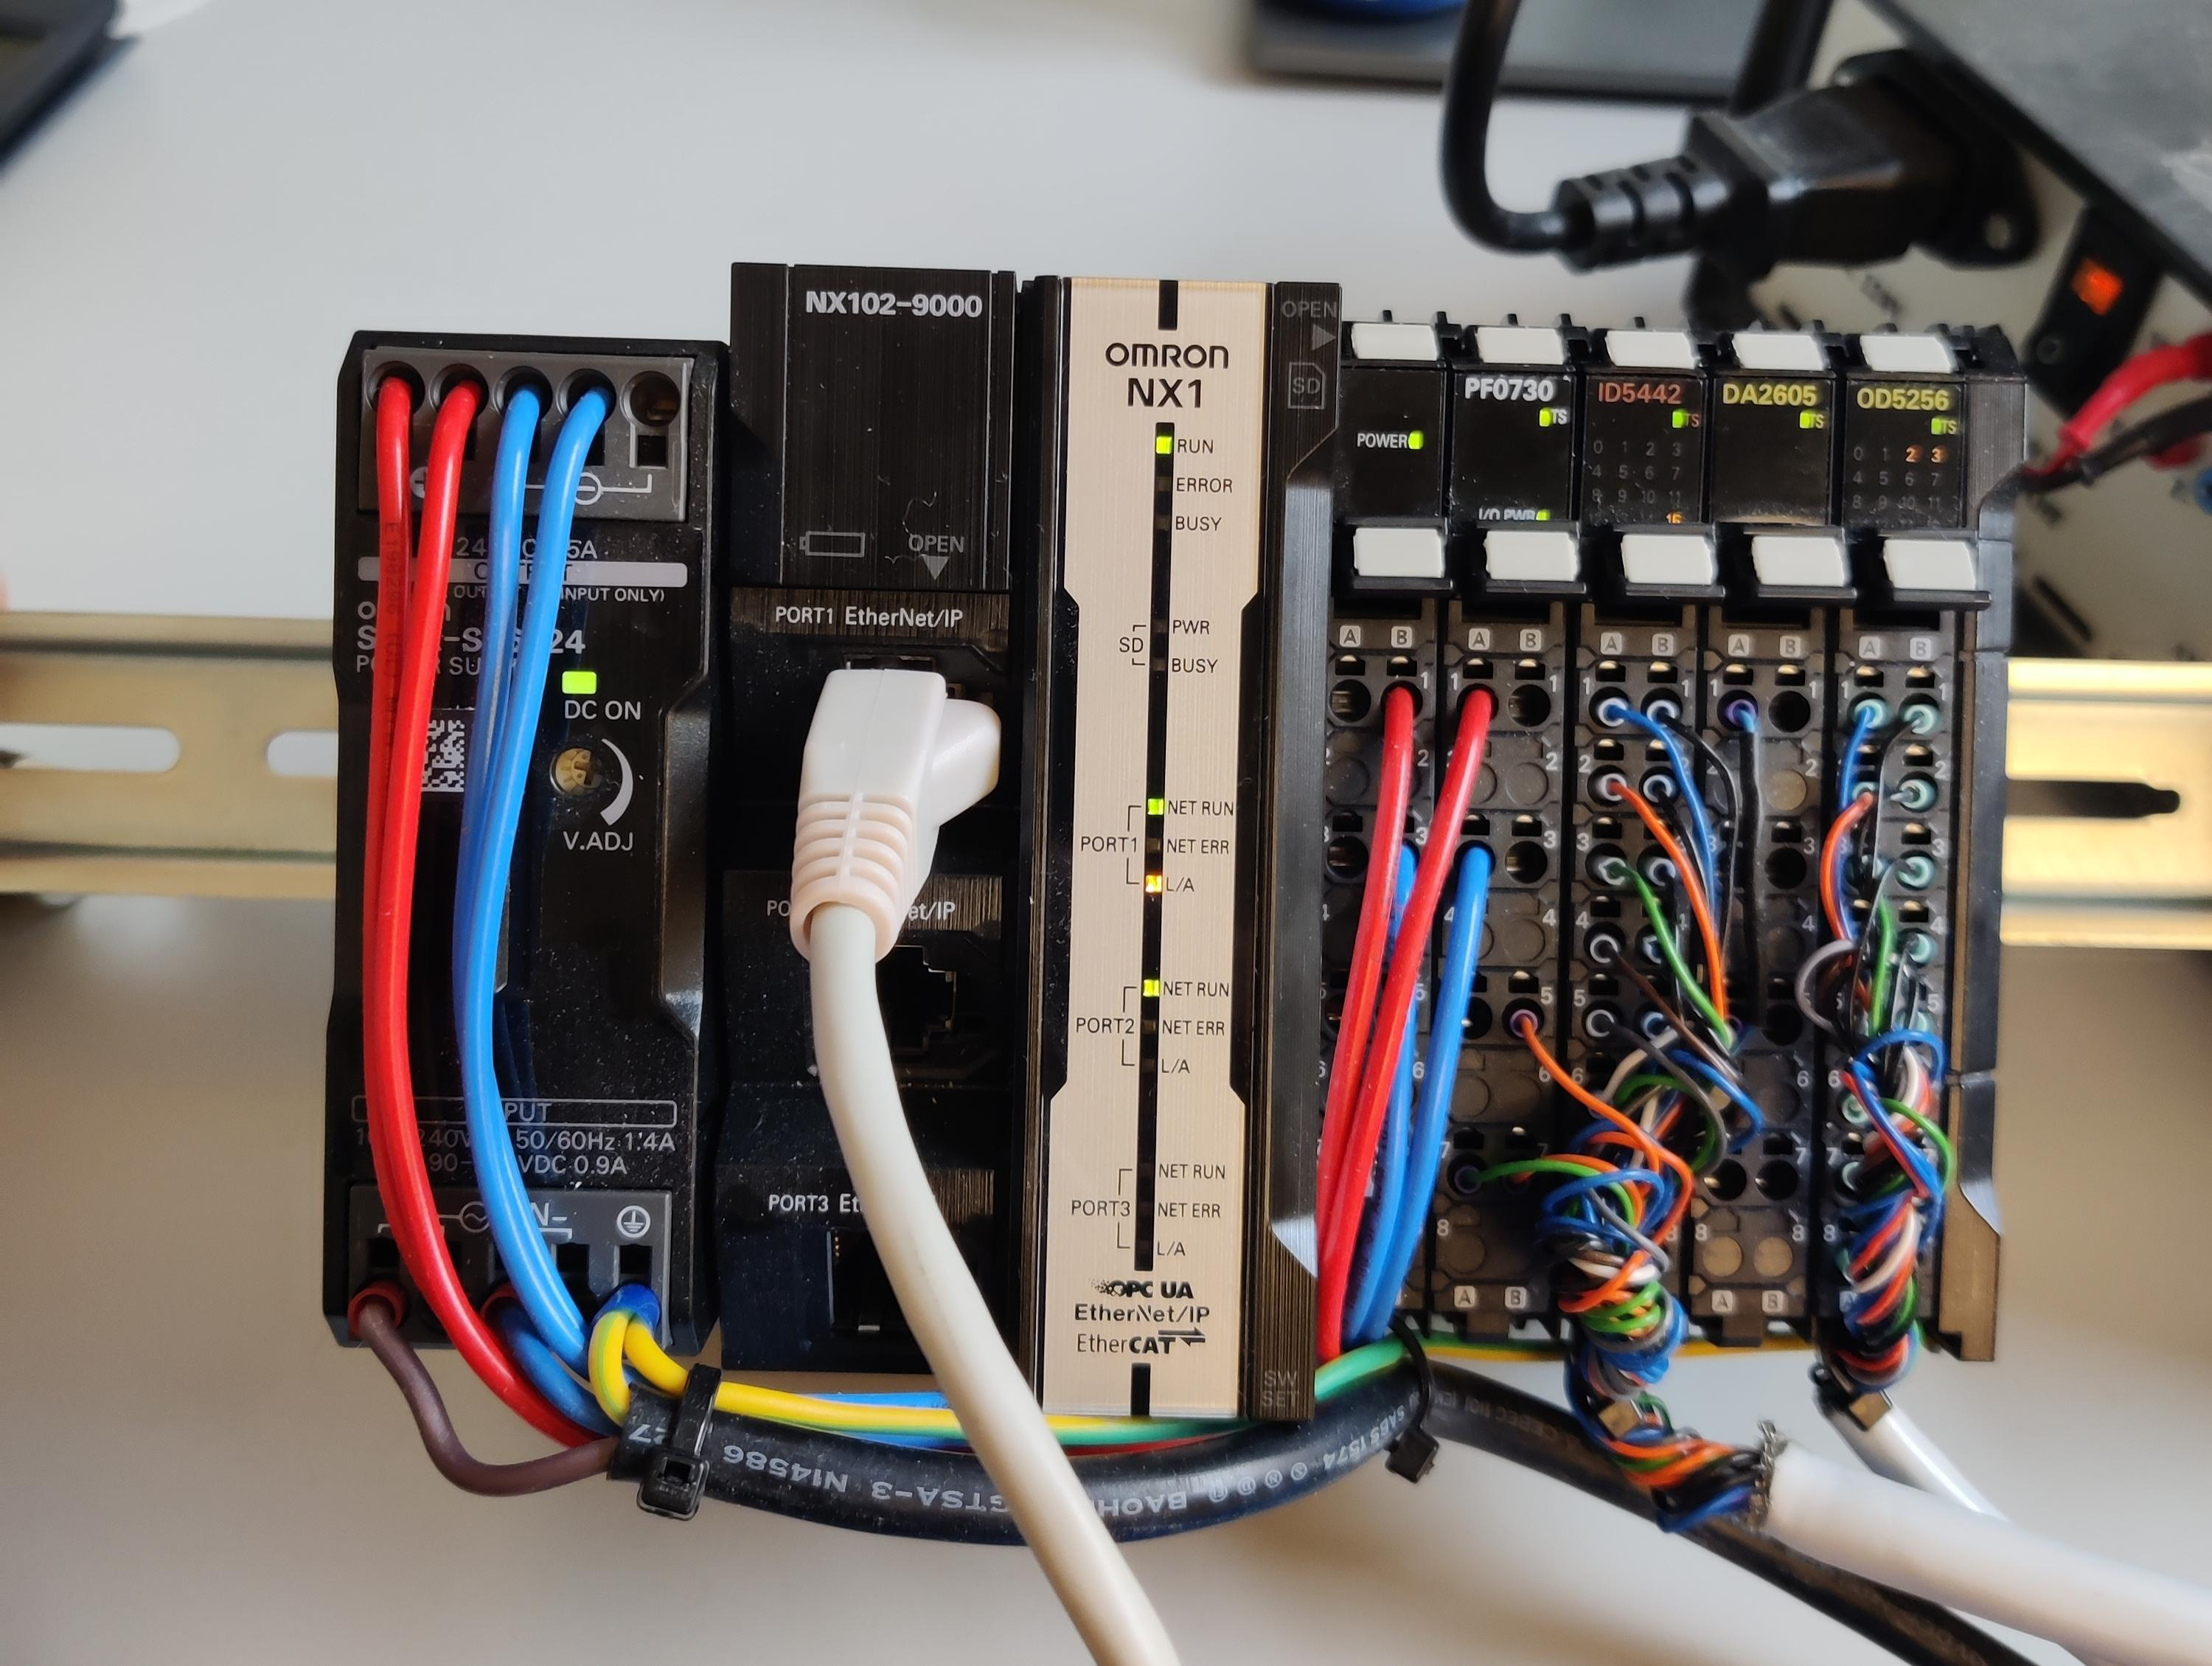
\includegraphics[scale=0.1]{figures/omron-pls.jpg}
    \caption{PLSen på Sanntidslaben.}
    \label{fig:omron-pls}
\end{figure}

I tillegg til dette finner dere vår kjære, vakre heismodell på pulten deres (se figur \ref{fig:Heis-modell}):


\begin{figure}[ht!]
    \centering
    \includegraphics[scale=.85]{figures/heis.PNG}
    \caption{Heis-modellen på Sanntidslaben.}
    \label{fig:Heis-modell}
\end{figure}

\subsection{Heismodellen}

Denne heismodellen består av en sjakt og en bevegelig heisstol. Det er denne vi skal få til å bevege seg i labopplegget. Over øverste etasje, og under nederste etasje er det montert endestoppbrytere, som vil kutte motorpådraget dersom heisen kjører utenfor sitt lovlige område. Dette er for å beskytte heisens motor mot skade. Om heisen skulle treffe en av endestoppene, må heisstolen manuelt skyves bort fra bryterne før man kan be motoren om et nytt pådrag. Dette er en beskyttelsemekanisme i hardware og skal ikke inngå i selve styresystemet som skal bli utviklet i denne labben.



\subsection{Motorstyringsboks}
Heisens pådrag kommer fra en motorstyringsenhet, den store svarte boksen som står ved siden av heismodellen i figur \ref{fig:Heis-modell}. Motorstyringsboksen er utstyrt med innebygd strømforsyning og kraftforsterker. Veien motoren skal gå settes ved et ekstra retningsbit i styringsboksens grensesnitt. Alt dette gjøres via funksjonskall i styringsprogrammet. Før dere gjør noe annet, skrur dere denne på, og passer på at den røde ledningen fra heisen er koblet til \verb|M+|, og den blå ledningen til \verb|M-|.


\subsection{Betjeningsboks}
Til slutt har dere en "betjeningsboks". Øverst på betjeningsboksen finnes en bryter som velger om datamaskinen eller PLSen skal styre heismodellen. Denne skal stå i "\verb|PLS|" gjennom hele labben.



Dersom man ser nærmere på betjeningsboksen, kan man se at den består av et etasjepanel, og et heispanel (se figur \ref{fig:paneler}):

Etasjepanelet finnes på oversiden av betjeningsboksen fra figur \ref{fig:Heis-modell}. Dette panelet blir brukt for å simulere bestillingsknappene for opp- og nedretning fra hver etasje.  Hver av knappene er utstyrt med lys som skal indikere om en bestilling er mottatt eller ei. Etasjepanelet har også ett lys for hver etasje for å indikere hvilken etasje heisen befinner seg i. Det finnes ingen direkte kopling mellom knappene og lyssignalet i elektronikken så lyset må settes av styringssystemet.

Heispanelet derimot, finner man på kortsiden av betjeningsboksen og representerer de knappene man forventer å finne inne i heisrommet til en vanlig heis. Her har man bestillingsknapper for hver etasje, samt en stoppknapp for nødstans. Alle knappene er utstyrt med lys som kan settes via styreprogrammet. I tillegg til knappene er panelet utstyrt med etasjeindikatorlys som kan settes via styreprogrammet og et lys, markert med "\verb|Dør Åpen|", som indikerer om heisdøren er åpen. Heispanelet har også en obstruksjonsbryter, som kan brukes for å simulere at en person blokkerer døren når den er åpen.
\begin{figure}[ht!]
    \centering

\resizebox{1\textwidth}{!}{\tikzset{every picture/.style={line width=0.75pt}} %set default line width to 0.75pt        


\tikzset{every picture/.style={line width=0.75pt}} %set default line width to 0.75pt        

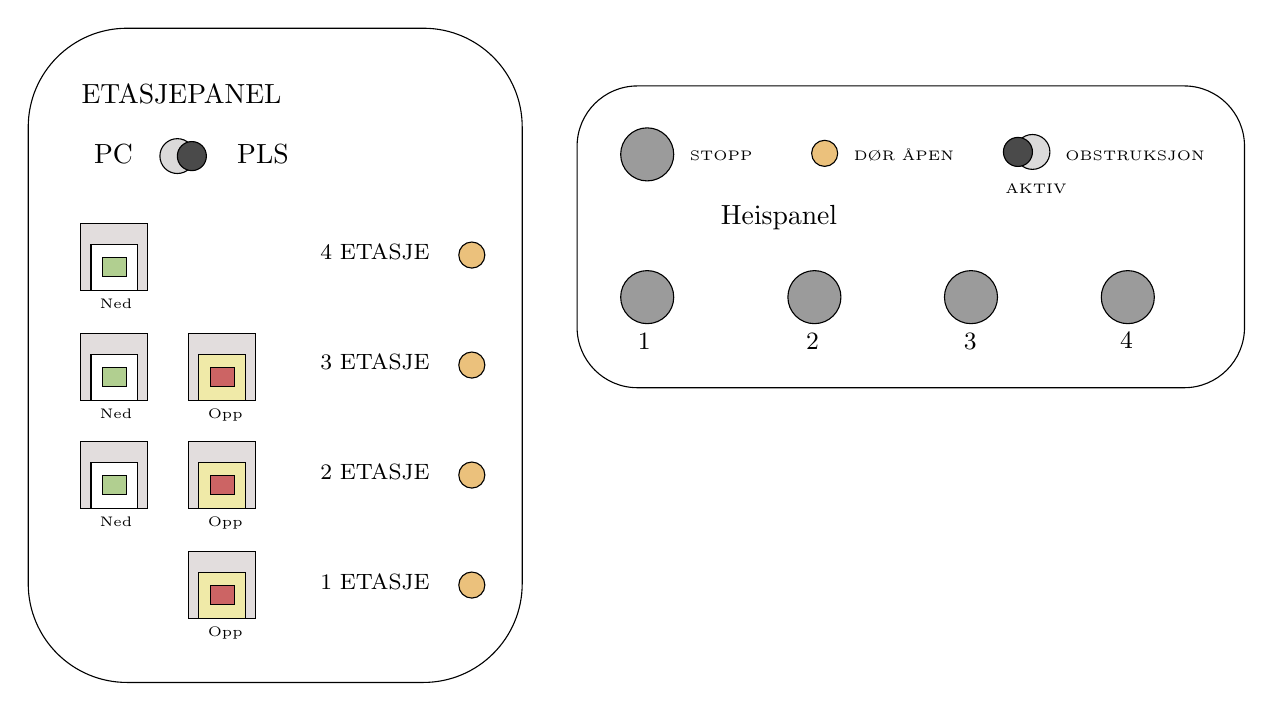
\begin{tikzpicture}[x=0.75pt,y=0.75pt,yscale=-1,xscale=1]
%uncomment if require: \path (0,386); %set diagram left start at 0, and has height of 386

%Rounded Rect [id:dp9950110832791259] 
\draw   (47.56,88.6) .. controls (47.56,62.31) and (68.87,41) .. (95.16,41) -- (237.96,41) .. controls (264.25,41) and (285.56,62.31) .. (285.56,88.6) -- (285.56,308.6) .. controls (285.56,334.89) and (264.25,356.2) .. (237.96,356.2) -- (95.16,356.2) .. controls (68.87,356.2) and (47.56,334.89) .. (47.56,308.6) -- cycle ;
%Shape: Circle [id:dp32702530949930675] 
\draw  [fill={rgb, 255:red, 219; green, 218; blue, 218 }  ,fill opacity=1 ] (111,102.6) .. controls (111,97.96) and (114.76,94.2) .. (119.4,94.2) .. controls (124.04,94.2) and (127.8,97.96) .. (127.8,102.6) .. controls (127.8,107.24) and (124.04,111) .. (119.4,111) .. controls (114.76,111) and (111,107.24) .. (111,102.6) -- cycle ;
%Shape: Circle [id:dp5550022005610891] 
\draw  [fill={rgb, 255:red, 74; green, 74; blue, 74 }  ,fill opacity=1 ] (119.4,102.6) .. controls (119.4,98.73) and (122.53,95.6) .. (126.4,95.6) .. controls (130.27,95.6) and (133.4,98.73) .. (133.4,102.6) .. controls (133.4,106.47) and (130.27,109.6) .. (126.4,109.6) .. controls (122.53,109.6) and (119.4,106.47) .. (119.4,102.6) -- cycle ;
%Rounded Rect [id:dp07742975412184872] 
\draw   (312,97.88) .. controls (312,81.82) and (325.02,68.8) .. (341.08,68.8) -- (604.48,68.8) .. controls (620.54,68.8) and (633.56,81.82) .. (633.56,97.88) -- (633.56,185.12) .. controls (633.56,201.18) and (620.54,214.2) .. (604.48,214.2) -- (341.08,214.2) .. controls (325.02,214.2) and (312,201.18) .. (312,185.12) -- cycle ;
%Shape: Circle [id:dp5584647222054995] 
\draw  [fill={rgb, 255:red, 155; green, 155; blue, 155 }  ,fill opacity=1 ] (333,101.78) .. controls (333,94.72) and (338.72,89) .. (345.78,89) .. controls (352.84,89) and (358.56,94.72) .. (358.56,101.78) .. controls (358.56,108.84) and (352.84,114.56) .. (345.78,114.56) .. controls (338.72,114.56) and (333,108.84) .. (333,101.78) -- cycle ;
%Shape: Circle [id:dp36378536676727435] 
\draw  [fill={rgb, 255:red, 235; green, 193; blue, 124 }  ,fill opacity=1 ] (425,101.28) .. controls (425,97.81) and (427.81,95) .. (431.28,95) .. controls (434.75,95) and (437.56,97.81) .. (437.56,101.28) .. controls (437.56,104.75) and (434.75,107.56) .. (431.28,107.56) .. controls (427.81,107.56) and (425,104.75) .. (425,101.28) -- cycle ;
%Shape: Circle [id:dp2626490795793748] 
\draw  [fill={rgb, 255:red, 219; green, 218; blue, 218 }  ,fill opacity=1 ] (523,100.6) .. controls (523,95.96) and (526.76,92.2) .. (531.4,92.2) .. controls (536.04,92.2) and (539.8,95.96) .. (539.8,100.6) .. controls (539.8,105.24) and (536.04,109) .. (531.4,109) .. controls (526.76,109) and (523,105.24) .. (523,100.6) -- cycle ;
%Shape: Circle [id:dp7325663462799819] 
\draw  [fill={rgb, 255:red, 74; green, 74; blue, 74 }  ,fill opacity=1 ] (517.4,100.6) .. controls (517.4,96.73) and (520.53,93.6) .. (524.4,93.6) .. controls (528.27,93.6) and (531.4,96.73) .. (531.4,100.6) .. controls (531.4,104.47) and (528.27,107.6) .. (524.4,107.6) .. controls (520.53,107.6) and (517.4,104.47) .. (517.4,100.6) -- cycle ;

%Shape: Circle [id:dp3804510595811603] 
\draw  [fill={rgb, 255:red, 155; green, 155; blue, 155 }  ,fill opacity=1 ] (333,170.56) .. controls (333,163.5) and (338.72,157.78) .. (345.78,157.78) .. controls (352.84,157.78) and (358.56,163.5) .. (358.56,170.56) .. controls (358.56,177.62) and (352.84,183.34) .. (345.78,183.34) .. controls (338.72,183.34) and (333,177.62) .. (333,170.56) -- cycle ;
%Shape: Circle [id:dp9317202699472626] 
\draw  [fill={rgb, 255:red, 155; green, 155; blue, 155 }  ,fill opacity=1 ] (413.56,170.56) .. controls (413.56,163.5) and (419.28,157.78) .. (426.34,157.78) .. controls (433.4,157.78) and (439.12,163.5) .. (439.12,170.56) .. controls (439.12,177.62) and (433.4,183.34) .. (426.34,183.34) .. controls (419.28,183.34) and (413.56,177.62) .. (413.56,170.56) -- cycle ;
%Shape: Circle [id:dp8967657062909633] 
\draw  [fill={rgb, 255:red, 155; green, 155; blue, 155 }  ,fill opacity=1 ] (489,170.56) .. controls (489,163.5) and (494.72,157.78) .. (501.78,157.78) .. controls (508.84,157.78) and (514.56,163.5) .. (514.56,170.56) .. controls (514.56,177.62) and (508.84,183.34) .. (501.78,183.34) .. controls (494.72,183.34) and (489,177.62) .. (489,170.56) -- cycle ;
%Shape: Circle [id:dp46875668862956843] 
\draw  [fill={rgb, 255:red, 155; green, 155; blue, 155 }  ,fill opacity=1 ] (564.56,170.56) .. controls (564.56,163.5) and (570.28,157.78) .. (577.34,157.78) .. controls (584.4,157.78) and (590.12,163.5) .. (590.12,170.56) .. controls (590.12,177.62) and (584.4,183.34) .. (577.34,183.34) .. controls (570.28,183.34) and (564.56,177.62) .. (564.56,170.56) -- cycle ;
%Shape: Circle [id:dp6506882141668844] 
\draw  [fill={rgb, 255:red, 235; green, 193; blue, 124 }  ,fill opacity=1 ] (255,150.28) .. controls (255,146.81) and (257.81,144) .. (261.28,144) .. controls (264.75,144) and (267.56,146.81) .. (267.56,150.28) .. controls (267.56,153.75) and (264.75,156.56) .. (261.28,156.56) .. controls (257.81,156.56) and (255,153.75) .. (255,150.28) -- cycle ;
%Shape: Circle [id:dp7349408120329506] 
\draw  [fill={rgb, 255:red, 235; green, 193; blue, 124 }  ,fill opacity=1 ] (255,203.28) .. controls (255,199.81) and (257.81,197) .. (261.28,197) .. controls (264.75,197) and (267.56,199.81) .. (267.56,203.28) .. controls (267.56,206.75) and (264.75,209.56) .. (261.28,209.56) .. controls (257.81,209.56) and (255,206.75) .. (255,203.28) -- cycle ;
%Shape: Circle [id:dp08591264771647289] 
\draw  [fill={rgb, 255:red, 235; green, 193; blue, 124 }  ,fill opacity=1 ] (255,256.28) .. controls (255,252.81) and (257.81,250) .. (261.28,250) .. controls (264.75,250) and (267.56,252.81) .. (267.56,256.28) .. controls (267.56,259.75) and (264.75,262.56) .. (261.28,262.56) .. controls (257.81,262.56) and (255,259.75) .. (255,256.28) -- cycle ;
%Shape: Circle [id:dp13492097445361106] 
\draw  [fill={rgb, 255:red, 235; green, 193; blue, 124 }  ,fill opacity=1 ] (255,309.28) .. controls (255,305.81) and (257.81,303) .. (261.28,303) .. controls (264.75,303) and (267.56,305.81) .. (267.56,309.28) .. controls (267.56,312.75) and (264.75,315.56) .. (261.28,315.56) .. controls (257.81,315.56) and (255,312.75) .. (255,309.28) -- cycle ;
%Shape: Square [id:dp9156786654213831] 
\draw  [fill={rgb, 255:red, 226; green, 221; blue, 221 }  ,fill opacity=1 ] (72.8,135) -- (105,135) -- (105,167.2) -- (72.8,167.2) -- cycle ;
%Shape: Rectangle [id:dp9366523430197387] 
\draw  [color={rgb, 255:red, 0; green, 0; blue, 0 }  ,draw opacity=1 ][fill={rgb, 255:red, 255; green, 255; blue, 255 }  ,fill opacity=1 ] (77.8,145.2) -- (100.24,145.2) -- (100.24,167.2) -- (77.8,167.2) -- cycle ;
%Shape: Rectangle [id:dp17647947769063999] 
\draw  [fill={rgb, 255:red, 177; green, 207; blue, 144 }  ,fill opacity=1 ] (83.24,151.6) -- (94.8,151.6) -- (94.8,160.8) -- (83.24,160.8) -- cycle ;
%Shape: Square [id:dp3110641273660344] 
\draw  [fill={rgb, 255:red, 226; green, 221; blue, 221 }  ,fill opacity=1 ] (124.8,188) -- (157,188) -- (157,220.2) -- (124.8,220.2) -- cycle ;
%Shape: Rectangle [id:dp3411082188269683] 
\draw  [fill={rgb, 255:red, 240; green, 234; blue, 168 }  ,fill opacity=1 ] (129.8,198.2) -- (152.24,198.2) -- (152.24,220.2) -- (129.8,220.2) -- cycle ;
%Shape: Rectangle [id:dp024921669891114773] 
\draw  [fill={rgb, 255:red, 204; green, 100; blue, 100 }  ,fill opacity=1 ] (135.24,204.6) -- (146.8,204.6) -- (146.8,213.8) -- (135.24,213.8) -- cycle ;
%Shape: Square [id:dp802085856449118] 
\draw  [fill={rgb, 255:red, 226; green, 221; blue, 221 }  ,fill opacity=1 ] (124.8,240) -- (157,240) -- (157,272.2) -- (124.8,272.2) -- cycle ;
%Shape: Rectangle [id:dp5915145699519246] 
\draw  [fill={rgb, 255:red, 240; green, 234; blue, 168 }  ,fill opacity=1 ] (129.8,250.2) -- (152.24,250.2) -- (152.24,272.2) -- (129.8,272.2) -- cycle ;
%Shape: Rectangle [id:dp03960973210916041] 
\draw  [fill={rgb, 255:red, 204; green, 100; blue, 100 }  ,fill opacity=1 ] (135.24,256.6) -- (146.8,256.6) -- (146.8,265.8) -- (135.24,265.8) -- cycle ;
%Shape: Square [id:dp831298532737776] 
\draw  [fill={rgb, 255:red, 226; green, 221; blue, 221 }  ,fill opacity=1 ] (124.8,293) -- (157,293) -- (157,325.2) -- (124.8,325.2) -- cycle ;
%Shape: Rectangle [id:dp15467787894146512] 
\draw  [fill={rgb, 255:red, 240; green, 234; blue, 168 }  ,fill opacity=1 ] (129.8,303.2) -- (152.24,303.2) -- (152.24,325.2) -- (129.8,325.2) -- cycle ;
%Shape: Rectangle [id:dp34679432751904793] 
\draw  [fill={rgb, 255:red, 204; green, 100; blue, 100 }  ,fill opacity=1 ] (135.24,309.6) -- (146.8,309.6) -- (146.8,318.8) -- (135.24,318.8) -- cycle ;
%Shape: Square [id:dp4723272264815428] 
\draw  [fill={rgb, 255:red, 226; green, 221; blue, 221 }  ,fill opacity=1 ] (72.8,240) -- (105,240) -- (105,272.2) -- (72.8,272.2) -- cycle ;
%Shape: Rectangle [id:dp07462637657852489] 
\draw  [color={rgb, 255:red, 0; green, 0; blue, 0 }  ,draw opacity=1 ][fill={rgb, 255:red, 255; green, 255; blue, 255 }  ,fill opacity=1 ] (77.8,250.2) -- (100.24,250.2) -- (100.24,272.2) -- (77.8,272.2) -- cycle ;
%Shape: Rectangle [id:dp5263621720064795] 
\draw  [fill={rgb, 255:red, 177; green, 207; blue, 144 }  ,fill opacity=1 ] (83.24,256.6) -- (94.8,256.6) -- (94.8,265.8) -- (83.24,265.8) -- cycle ;
%Shape: Square [id:dp4171956285217089] 
\draw  [fill={rgb, 255:red, 226; green, 221; blue, 221 }  ,fill opacity=1 ] (72.8,188) -- (105,188) -- (105,220.2) -- (72.8,220.2) -- cycle ;
%Shape: Rectangle [id:dp8897782495872741] 
\draw  [color={rgb, 255:red, 0; green, 0; blue, 0 }  ,draw opacity=1 ][fill={rgb, 255:red, 255; green, 255; blue, 255 }  ,fill opacity=1 ] (77.8,198.2) -- (100.24,198.2) -- (100.24,220.2) -- (77.8,220.2) -- cycle ;
%Shape: Rectangle [id:dp3645531927882917] 
\draw  [fill={rgb, 255:red, 177; green, 207; blue, 144 }  ,fill opacity=1 ] (83.24,204.6) -- (94.8,204.6) -- (94.8,213.8) -- (83.24,213.8) -- cycle ;

% Text Node
\draw (72,67) node [anchor=north west][inner sep=0.75pt]   [align=left] {ETASJEPANEL};
% Text Node
\draw (78,96) node [anchor=north west][inner sep=0.75pt]   [align=left] {PC};
% Text Node
\draw (147,96) node [anchor=north west][inner sep=0.75pt]   [align=left] {PLS};
% Text Node
\draw (380.05,124.81) node [anchor=north west][inner sep=0.75pt]   [align=left] {Heispanel};
% Text Node
\draw (444.05,97.81) node [anchor=north west][inner sep=0.75pt]  [font=\tiny] [align=left] {DØR ÅPEN};
% Text Node
\draw (546.05,98.81) node [anchor=north west][inner sep=0.75pt]  [font=\tiny] [align=left] {OBSTRUKSJON};
% Text Node
\draw (365.05,98.81) node [anchor=north west][inner sep=0.75pt]  [font=\tiny] [align=left] {STOPP};
% Text Node
\draw (517.05,114.81) node [anchor=north west][inner sep=0.75pt]  [font=\tiny] [align=left] {AKTIV};
% Text Node
\draw (340.05,186.81) node [anchor=north west][inner sep=0.75pt]  [font=\small] [align=left] {1};
% Text Node
\draw (421.05,186.81) node [anchor=north west][inner sep=0.75pt]  [font=\small] [align=left] {2};
% Text Node
\draw (497.05,186.81) node [anchor=north west][inner sep=0.75pt]  [font=\small] [align=left] {3};
% Text Node
\draw (572.34,186.34) node [anchor=north west][inner sep=0.75pt]  [font=\small] [align=left] {4};
% Text Node
\draw (187,144) node [anchor=north west][inner sep=0.75pt]  [font=\footnotesize] [align=left] {4 ETASJE};
% Text Node
\draw (187,197) node [anchor=north west][inner sep=0.75pt]  [font=\footnotesize] [align=left] {3 ETASJE};
% Text Node
\draw (187,250) node [anchor=north west][inner sep=0.75pt]  [font=\footnotesize] [align=left] {2 ETASJE};
% Text Node
\draw (187,303) node [anchor=north west][inner sep=0.75pt]  [font=\footnotesize] [align=left] {1 ETASJE};
% Text Node
\draw (80.8,170.2) node [anchor=north west][inner sep=0.75pt]  [font=\tiny] [align=left] {Ned};
% Text Node
\draw (80.8,223.2) node [anchor=north west][inner sep=0.75pt]  [font=\tiny] [align=left] {Ned};
% Text Node
\draw (80.8,275.2) node [anchor=north west][inner sep=0.75pt]  [font=\tiny] [align=left] {Ned};
% Text Node
\draw (132.8,223.2) node [anchor=north west][inner sep=0.75pt]  [font=\tiny] [align=left] {Opp};
% Text Node
\draw (132.8,275.2) node [anchor=north west][inner sep=0.75pt]  [font=\tiny] [align=left] {Opp};
% Text Node
\draw (132.8,328.2) node [anchor=north west][inner sep=0.75pt]  [font=\tiny] [align=left] {Opp};


\end{tikzpicture}}
    \caption{Etasje- og Heispanel i Sanntidslabben}
    \label{fig:paneler}
\end{figure}



\section{Introduksjon - Programmering av PLS}

Måten man programmerer PLSer på er standarisert og følger en industristandard kalt \verb|IEC 61131-3|. Denne standarden definerer flere forskjellige måter man kan programmere/fortelle en PLS hva den skal gjøre. Fire av de vanligste av disse er:

\begin{itemize}
    \item \verb|Stigediagram (LD)|, eller "Ladder diagram": er et grafisk programmeringsspråk, hvor man lager linjer som representerer programflyt, hvor linjene kan ha brytere som representerer kontrollstrukturer.
    
    \item \verb|Funksjonsblokkdiagram (FBD)|: er også et grafisk programmeringsspråk, men her trekker man koblinger mellom utgangen på blokker inn i inngangene til andre blokker. 
    \item \verb|Strukturerert tekst (ST)|: er et programmeringsspråk som faktisk bruker tekjst - som navnet tilsier. Det ligner på et språk som heter "PASCAL".
    
    \item \verb|Sekvensielle funksjonsdiagram (SFC)| eller "Sequential function chart": er nok et grafisk programmeringsspråk, men har i tillegg noen elementer for å kunne blande sekvensielle operasjoner med parallelle operasjoner.
\end{itemize}

For å programmere i Sysmac skal dere bruke den utdelte manualen, ved navn "Sysmac Studio Version 1 Operation Manual", samt kurskompendiet, som begge to finnes i organisasjonen til TTK4235 på GitHub. Ta en titt i disse ressursene før dere eventuelt ber om hjelp, ettersom alt man trenger å vite står her. I programmet Sysmac, som skal være installert på alle Sanntids-PCene sine Windows-partisjoner, har man blant annet muligheten til følgende:

\begin{itemize}
    \item Sette opp og organisere prosjekter
    \item Konfigurere hardware
    \item Programmere blokker
    \item Laste ned program til PLSen
    \item Debugge programmet
\end{itemize}

Av de forskjellige programmeringstypene skal vi kun benytte oss av stigediagrammer i denne laben.

\subsection{Innføring i bruken av Sysmac}
Når dere skal programmere NX102-9000 er det første man gjør å åpne Sysmac Studio fra Windows-partisjonen på PCene på Sanntidssalen. Deretter må man sjekke at man er tilkoplet PLSen. Dette gjør man ved å trykke på "Connect to Device" fra hovedmenyen. Her velger man alternativet "Direct Connection Via Ethernet", og trykker slik at boksen "Transfer from Device" er tom, og deretter "Connect".

%  Dersom man får en feilmelding her, kan det hende at ikke riktig enhet er valgt i "DirectEthernetUtility" som følger med programvaren. Dette kan i såfall løses ved å følge det som står i "1.8 Opprette et nytt prosjekt Online" i Kurskompendiet. Kort forklart innebærer dette følgende:

% \begin{itemize}
%     \item Åpne startmenyen og finn mappen "Omron", den skal ligge under "C:/ProgramData/textbackslash Omron/".
%     \item Under "Communications", åpne programmet "DirectEthernetUtility".
%     \item 
% \end{itemize}

Nå skal man være tilkoplet PLSen, hvis du ikke er det enda, trykk på den gule trekanten som heter "Online" i verktøylinja. Nå kan det hende at dere må enten skrive inn eller velge brukernavn og passord. I begge tilfellene skriver dere inn "TTK4235" som brukernavn, og "Sanntid15" som passord. Før vi går videre skal vi slette minnet som er på PLSen, slik at dere får det man kaller for en "fresh start" på engelsk. Trykk derfor på det runde hjulet i verktøylinja som heter "Synchronize". Her velger dere alternativet "Transfer To Controller", og deretter "Yes". Nå har vi overført et blankt program til PLSen.\\

Hvis vi så trykker på "Configurations and Setup" i "Multiview Explorer" på venstre side av brukergrensesnittet, deretter "CPU/Expansion Racks", og så "CPU Rack". Da dukker det opp et bilde av PLSen vår uten såkalte "expansions" til høyre for "Multiview Explorer". Høyreklikk på denne og velg alternativet "Compare and Merge with Actual Unit Configuration", og deretter "Apply Actual Unit Configuration".\\

Nå skal fabrikkinstillingene fra PLSen være matet inn i Sysmac, slik at vi kan begynne å programmere. Dette innebærer blant annet at Sysmac nå kjenner til det fysiske PLS-oppsettet vårt, noe som gjør det enkelt å tilordne inngangene og utgangene til PLSen med de tilsvarende til heismodellen, noe som er selve kjernen i PLS-programmering. Vær bevisst på det at vi må kople oss av PLSen for å kunne programmere, og dette gjøres ved å trykke på den gule trekanten med strek over i verktøylinja, som heter "Offline". Ikke kople deg av helt enda.

\subsubsection{Tilordning av I/O}
Hvis vi så trykker på "Configurations and Setup" i "Multiview Explorer" på venstre side av brukergrensesnittet, deretter "I/O Map", og så "NX Bus Master", så ser vi det at vi nå har importert hardware-oppsettet til PLSen fra dens minne, slik at det fysiske oppsettet vårt speiles i Sysmac. Vi kan derfor se de fire enhetene som er koplet til PLSen, altså NX-PF0730, NX-ID5442, NX-DA2605, samt NX-OD5256. Hvis vi nå kopler oss fra PLSen ved å trykke på "Offline", og deretter høyreklikker på "NX Bus Master", og så velger "Create Device Variable", så vil vi definere variabler basert på inn- og utgangene våre. Dette vil være nyttig senere når vi skal programmere. Hvis vi klikker på de fire NX-modulene under NX Bus Master vil vi få opp kartet over I/O-portene våre.

De digitale inngangene og utgangene til PLSen er koplet til heismodellen på følgende måte:

\begin{center}
 {\begin{tabular}{|c| c|} 
 \hline
 \textbf{Port} & \textbf{Beskrivelse} \\ 
 \toprule
 \verb|Input Bit 00| & Obstruksjon \\ 
 \hline
 \verb|Input Bit 01| & Stopp-knapp \\ 
 \hline
 \verb|Input Bit 02| & H1 - Bestillingsknapp nr. 1 inne i heisen \\ 
 \hline
 \verb|Input Bit 03| & H1 - Bestillingsknapp nr. 2 inne i heisen \\ 
 \hline
 \verb|Input Bit 04| & H1 - Bestillingsknapp nr. 3 inne i heisen \\ 
 \hline
 \verb|Input Bit 05| & H1 - Bestillingsknapp nr. 4 inne i heisen \\ 
 \hline
 \verb|Input Bit 06| & Opp-knapp i etasje 1 \\ 
 \hline
 \verb|Input Bit 07| & Opp-knapp i etasje 2 \\ 
 \toprule
 
 \verb|Input Bit 08| & Ned-knapp i etasje 2 \\ 
 \hline
 \verb|Input Bit 09| & Opp-knapp i etasje 3 \\ 
 \hline
 \verb|Input Bit 10| & Ned-knapp i etasje 3\\ 
 \hline
 \verb|Input Bit 11| & Ned-knapp i etasje 4 \\ 
 \hline
 \verb|Input Bit 12| & Føler 1. etasje \\ 
 \hline
 \verb|Input Bit 13| & Føler 2. etasje \\ 
 \hline
 \verb|Input Bit 14| & Føler 3. etasje \\ 
 \hline
 \verb|Input Bit 15| & Føler 4. etasje \\ 
 \toprule
 
 \verb|Output Bit 00| & DIR - Retning på motor (Opp=0, Ned=1) \\ 
 \hline
 \verb|Output Bit 01| & Lys i stopp-knapp \\ 
 \hline
 \verb|Output Bit 02| & Lys i bestillingsknapp nr. 1 \\ 
 \hline
 \verb|Output Bit 03| & Lys i bestillingsknapp nr. 2 \\ 
 \hline
 \verb|Output Bit 04| & Lys i bestillingsknapp nr. 3\\ 
 \hline
 \verb|Output Bit 05| & Lys i bestillingsknapp nr. 4\\ 
 \hline
 \verb|Output Bit 06| & Lys i opp-knapp i etasje 1 \\ 
 \hline
 \verb|Output Bit 07| & Lys i opp-knapp i etasje 2 \\ 
 \toprule
 
 \verb|Output Bit 08| & Lys i ned-knapp i etasje 2 \\ 
 \hline
 \verb|Output Bit 09| &Lys i opp-knapp i etasje 3 \\ 
 \hline
 \verb|Output Bit 10| & Lys i ned-knapp i etasje 3\\ 
 \hline
 \verb|Output Bit 11| & Lys i ned-knapp i etasje 4\\ 
 \hline
 \verb|Output Bit 12| & Lys i indikator for åpen dør \\ 
 \hline
 \verb|Output Bit 13| & Ubrukt \\ 
 \hline
 \verb|Output Bit 14| &Etasjeindikator bit 1 \\ 
 \hline
 \verb|Output Bit 15| &Etasjeindikator bit 2 \\ 
 \toprule
\end{tabular}}
\end{center}

Fra tabellen over, kan man se at man bare har to bit for å sette etasjeindikatorlysene. Dette er for spare utganger på PLSen. I vårt tilfelle, er lyset kodet slik:

\begin{center}
 {\begin{tabular}{|c| c| c|} 
 \hline
 \textbf{Bit 2} & \textbf{Bit 1} & \textbf{Etasjeindikator lys} \\ 
 \toprule
 0 & 0 & Etasje 1 \\ 
 \hline
 0 & 1 & Etasje 2 \\
 \hline
 1 & 0 & Etasje 3 \\
 \hline
 1 & 1 & Etasje 4 \\
 \toprule
\end{tabular}}
\end{center}

Sørg for at du er koplet fra PLSen, og gi passende navn til variablene i "I/O Map" ved å endre på feltet "Variable". Eksempler på navn kan være "DI00", altså forkortelsen for "Digital Input 00", til "Input Bit 00". Her hører "NX-ID5442" til de digitale inngangene, og "NX-OD5256" til de digitale utgangene. Vi har også to analoge utganger fra "NX-DA2605", hvorav vi kun bryr oss om den første, altså "Ch1 Analog Output Value". Denne styrer pådragssignalet til heismotoren, og er mellom 0 og 5V, alt ettersom hvilken av de heksadesimale eller desimale verdiene man gir utgangen fra den følgende tabellen:

\begin{center}
 {\begin{tabular}{|c| c| c|} 
 \hline
 \textbf{Heksadesimal verdi} & \textbf{Desimal verdi} & \textbf{Spenningsverdi} \\ 
 \toprule
 \verb|W#16#0000| & 0 & 0.0 \si{\V} \\ 
 \hline
 \verb|W#16#3DFF| & 15871 & 2.5 \si{\V}  \\
 \hline
 \verb|W#16#7EFF| & 32511 & 5.0 \si{\V}  \\

 \toprule
\end{tabular}}
\end{center}

Kople til PLSen ved å trykke på "Online", og trykk så på "Synchronize" og deretter "Transfer To Controller" for å synkronisere det vi har gjort i Sysmac med PLSen. Trykk "Yes" i de påfølgende dialogboksene. Sørg nå for at du er i "I/O Map". Dersom du nå trykker på knappene/bryterne på heisboksen, vil du se at de tilhørende inngangene går fra "False" til "True" under feltet "Value". I tillegg, sørg for at heisen er i nederste posisjon, slik at "Input Bit 12" er "True". Sjekk også at "Output Bit 00" er "False". Prøv nå å skrive 15871 til "Value"-feltet til "Ch1 Analog Output Value", altså den første porten til NX-DA2605. Du vil nå kunne se at heisen beveger seg oppover. Skriv 0 til dette feltet slik at motoren stopper, før du går videre.

\subsubsection{Utvikling og flashing av software}
Nå skal vi introdusere hvordan man kan programmere PLSen. På venstre hånd av Sysmac, i "Multiview Explorer", klikker vi derfor på "Programming", så "POUs", "Programs", "Program0", og så til slutt "Section0". Her får vi opp programmet vårt, slik det skal være flashet hos PLSen. Akkurat nå skal diagrammet være helt tomt, dersom dere har fulgt guiden til nå. Vi minner på at vi kun kan endre på diagrammet når vi er offline, altså ikke koplet til PLSen. Kople dere derfor av PLSen nå. \\

Vi skal nå lage et kjempeenkelt program, som skal gi dere litt intuisjon for hvordan man gjør stigeprogrammering i Sysmac. Dette skal deretter flashes til PLSen. Før dere gjør oppgavene i denne laben anbefaler vi dere å lese "Section 4 Programming" i databladet, da særlig "4-5 Programming Ladder Diagrams". Skjermbildet som dere skal se i Sysmac nå er vist i figur \ref{fig:empty_rung}.

\begin{figure}[ht]
    \centering
    \hspace*{-2cm}
    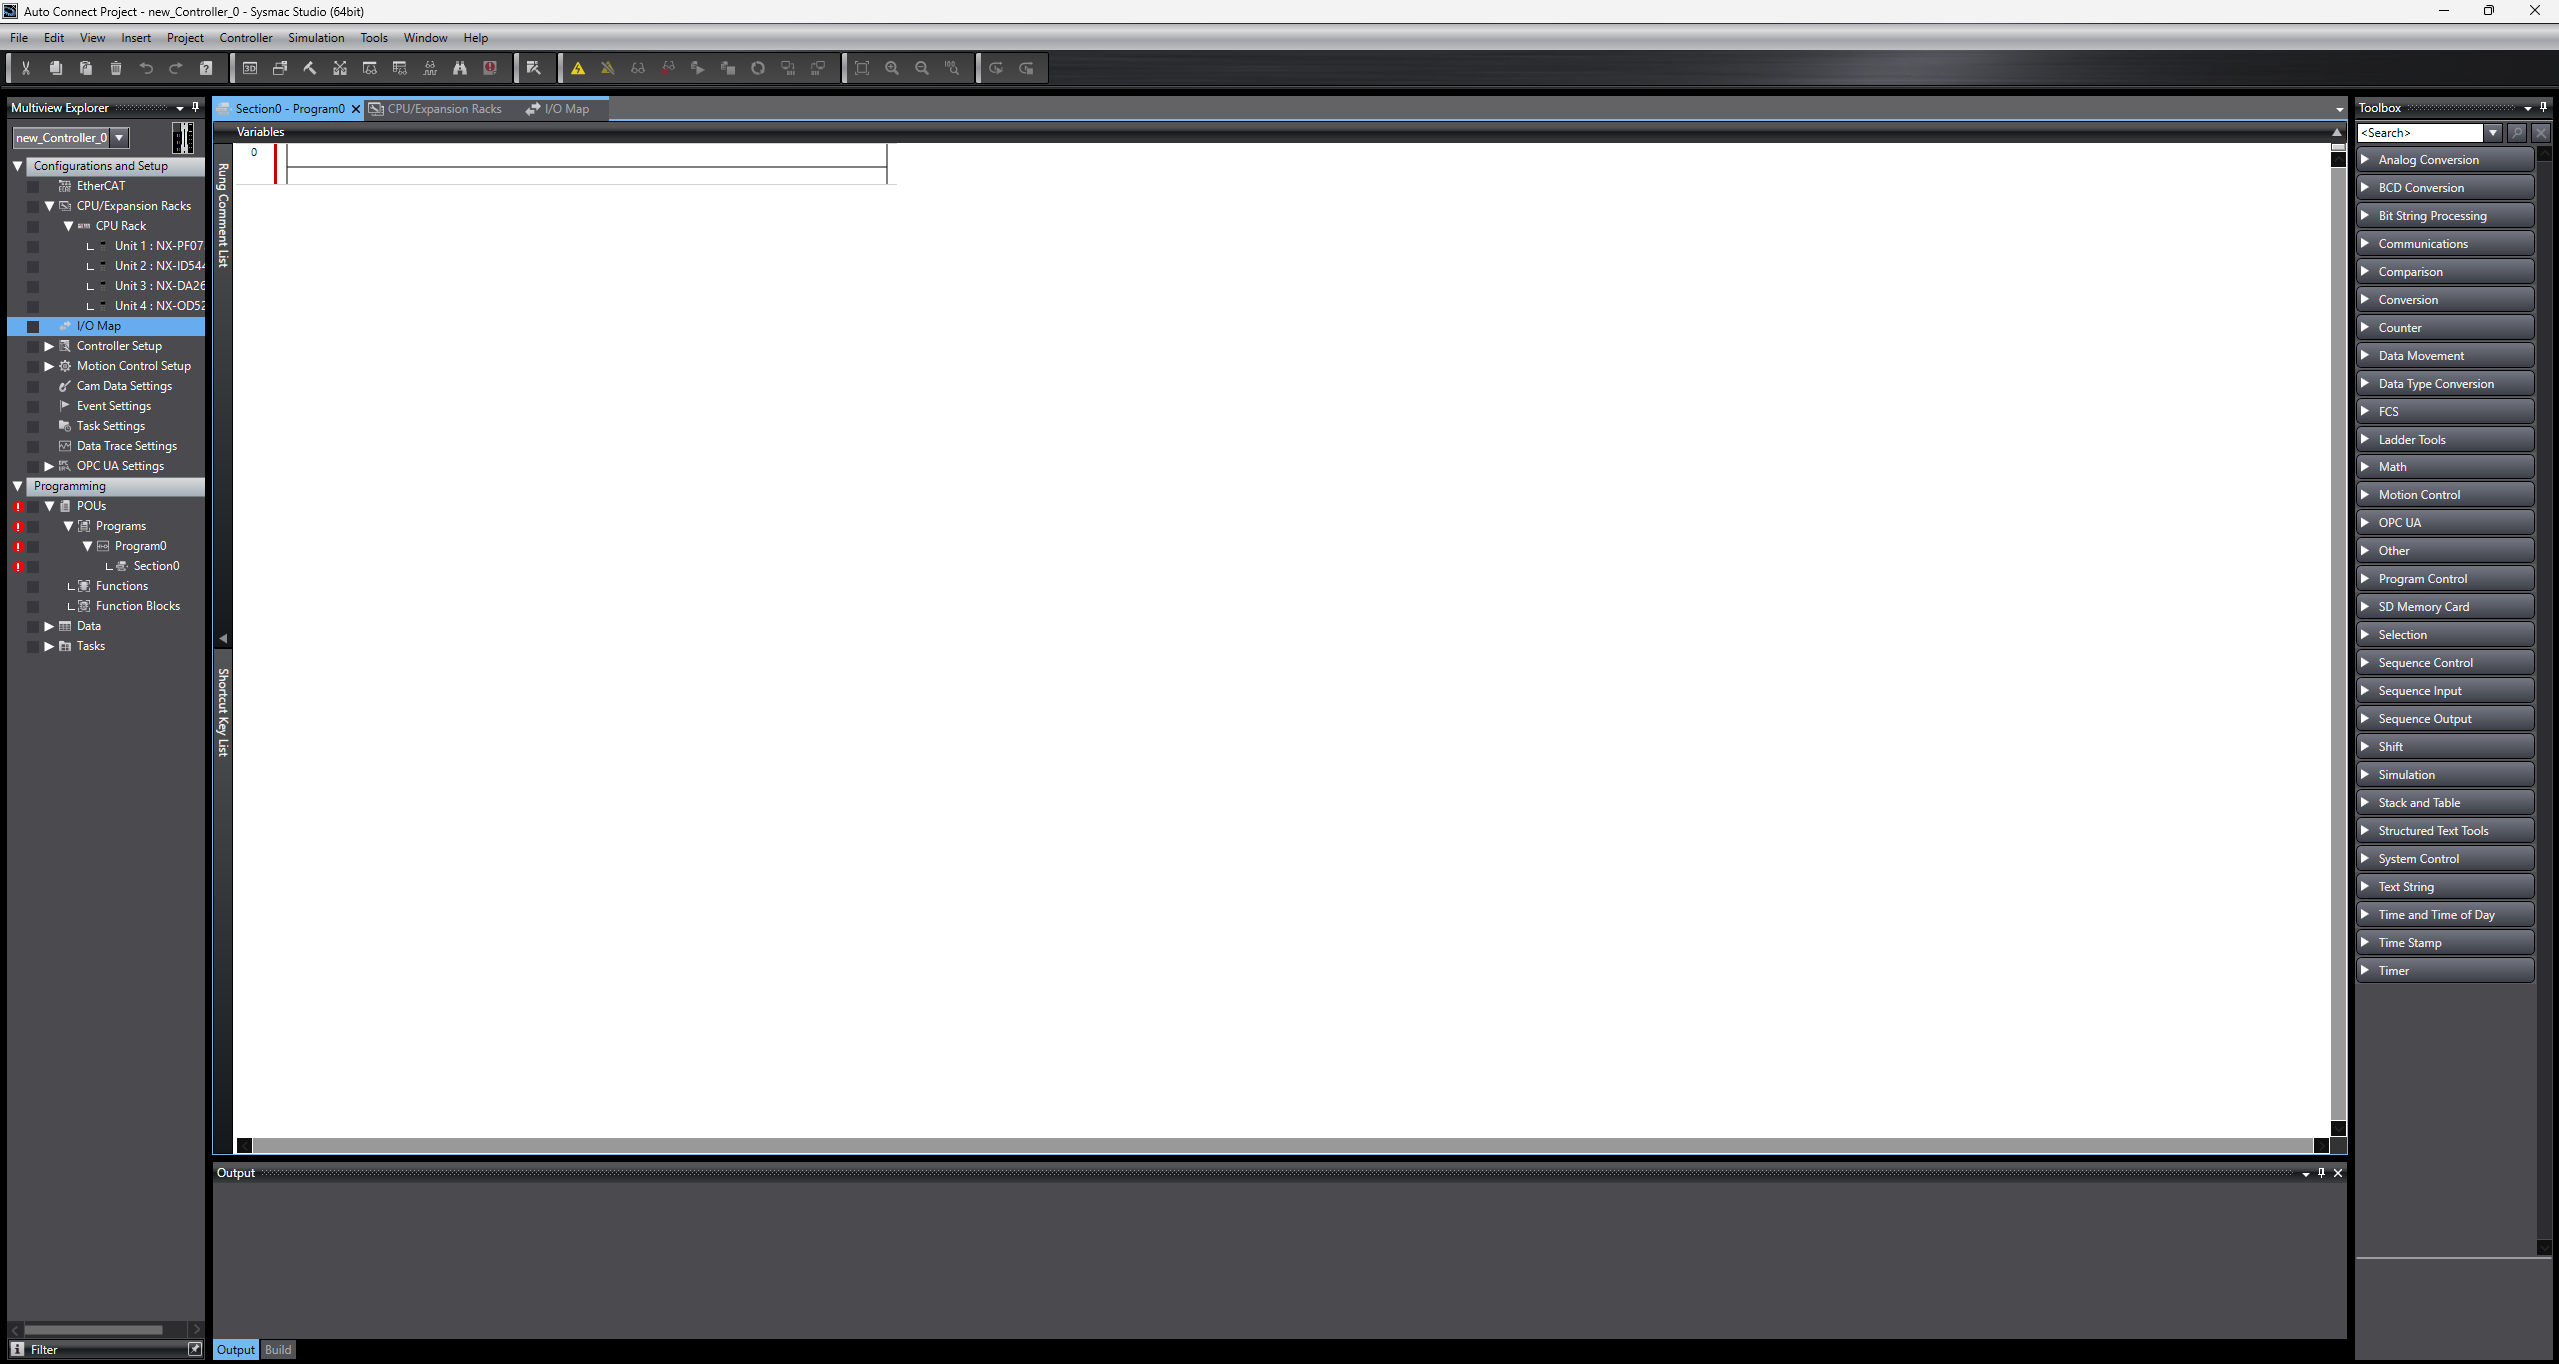
\includegraphics[scale=0.275]{figures/empty_rung.png}
    \caption{Programmeringsområdet vårt med tomt stigetrinn.}
    \label{fig:empty_rung}
\end{figure}

Dere ser nå et stort hvitt felt med det vi i stigeprogrammering kaller for et trinn (eller "rung" på engelsk) helt øverst til venstre. Det er i slike trinn man gjør programmeringen. Ved å høyreklikke på det får man opp en del valg, som for eksempel å lage flere trinn (dersom man høyreklikker helt til venstre på trinnet), eller som å sette inn elementer i trinnet (høyre del). Helt til høyre, ved siden av programmeringsfeltet, har vi "Toolbox". Her har du alle funksjoner du kan trenge å bruke til stigeprogrammering. Vi skal her og nå lage et kjempeenkelt program som kun skal sette lyset i indikatoren for åpen dør, dersom obstruksjonsbryteren er aktiv.\\

Det første vi gjør er å velge den inngangen vi ønsker. Vi høyreklikker derfor på trinnet, og velger "Insert Input", og skriver inn "DI00", dersom dette er navnet vi ga til inngangen for obstruksjonsbryteren. Deretter trykker vi på trinnet igjen og velger "Function", og skriver deretter inn "MOVE" for å velge riktig "Function". Det denne gjør er at når feltet "EN" går høy, settes det som står på "In" på "Out". Derfor skriver vi "1" på "In", og "DO12" på "Out", ettersom det er dette vi har kalt utgangen for lysindikatoren for åpen dør. Nå har programmert slik at lyset skrur seg på når vi skrur på bryteren, og vi må programmere slik at det skrur seg av når obstruksjonsbryteren ikke lenger er aktiv. Lag derfor et nytt trinn ved å høyreklikke på den venstre delen av det første trinnet vårt, og deretter "Insert Rung Below". Nå kan du lage akkurat samme struktur som tidligere. Deretter høyreklikker du på den nye inputen og velger "Invert", og så velger "0" i stedet for "1" på "In". Nå er det enkle programmet vårt ferdig, og det bør se ut som i figur \ref{fig:full_rung}.

\begin{figure}[ht]
    \centering
    \hspace*{-2cm}
    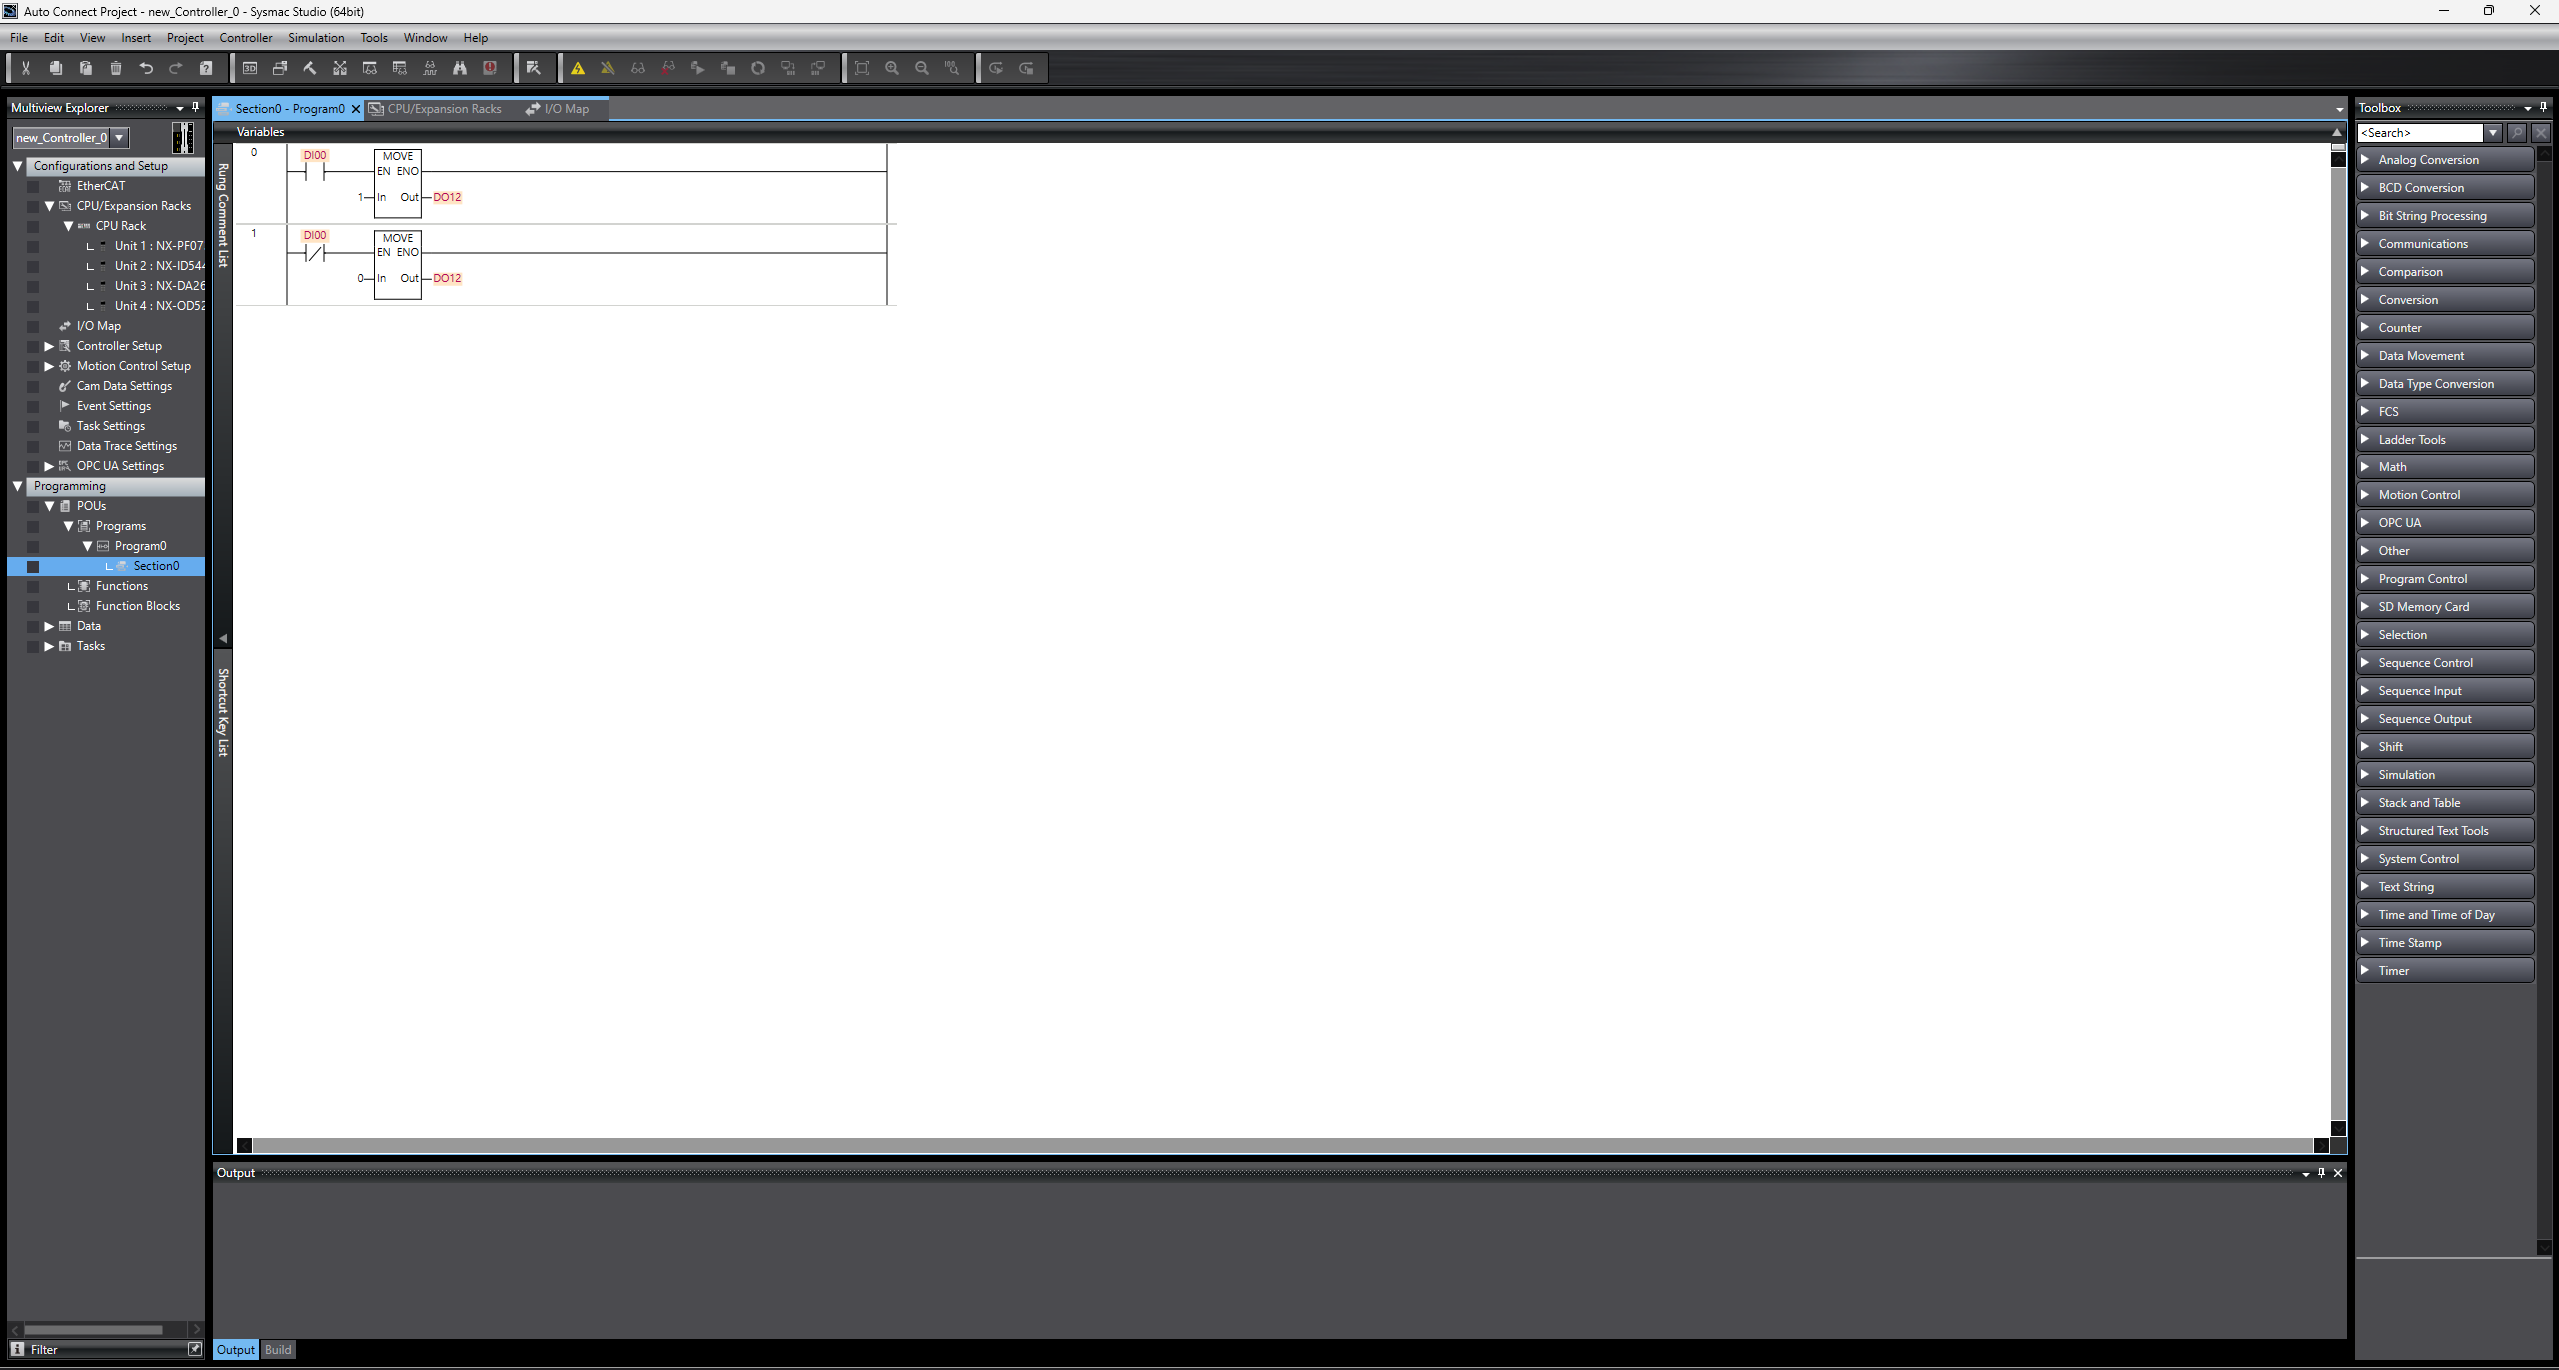
\includegraphics[scale=0.275]{figures/full_rung.png}
    \caption{Programmeringsområdet vårt med stigediagram.}
    \label{fig:full_rung}
\end{figure}

Så trykker vi på "Project", og deretter "Build Controller" i menylinja helt øverst, for å sjekke at programmet vårt ikke har noen feil. Dersom dette viser seg å stemme, kan vi kople oss til PLSen med "Online", og deretter flashe programmet vårt til PLSen ved å trykke på "Synchronize", og deretter "Transfer to Controller" i den påfølgende dialogboksen. Nå må vi sjekke at PLSen er i "RUN Mode". Dette er et symbol til høyre for "Online" på verktøylinja. Hvis denne lar seg trykke på, gjør dette, og hvis den allerede er grå, så er vi i riktig modus. Hvis vi nå trykker på obstruksjonsbryteren, så vil lyset som indikerer at døren er åpen lyse.\\

Nå har dere fått en liten innføring i Sysmac, og i oppgavene som kommer skal dere få lage et litt mer komplisert program, basert på god bruk av de utdelte databladene. Hvis dere har problemer underveis, anbefaler vi dere å sjekke appendiksen. Dersom dere ikke klarer å løse problemet med dette, sjekk det utdelte databladet eller kurskompendiet. Dersom dette ikke fungerer, spør en studass. Dersom dette ikke fungerer, ta en gåtur rundt Hovedbygget for å klarne tankene. Prøv deretter på nytt.
\end{alphasection}

\setcounter{section}{0}